\documentclass[T0_MEM]{subfiles}
\linespread{1.1}
\begin{document}

\section{Appendix B -- Out-of-sample forecasts}
\label{sec:more_countries}
In this section we present the results of our study
               performed in nine additional developed countries.

\newpage % ---------------------------
\subsection{Out-of-sample forecasts: Australia, Male population, 1960--2014}
\begin{table}[!ht]
\centering
\caption{Forecast accuracy measures aggregated over 16 scenarios in the 1960--2014 period} 
\label{tbl:res_AUS}
\scalebox{0.9}{
\begin{tabular}{lccccccc}
  \toprule
Model & ME & MAE & MAPE & sMAPE & sMRAE & MASE & GC \\ 
  \midrule
M.Random-Walk w Drift &  0.62 (5) &  0.64 (5) &  2.51 (5) &  2.56 (5) & 100.00 (6) &  3.21 (5) & (6) \\ 
  Lee-Carter &  0.55 (4) &  0.58 (4) &  2.26 (4) &  2.30 (4) &  96.03 (5) &  2.91 (4) & (4) \\ 
  Hyndman-Ullah &  0.48 (3) &  0.51 (3) &  2.11 (3) &  2.14 (3) &  92.80 (4) &  2.64 (3) & (3) \\ 
  Renshaw-Haberman &  0.83 (6) &  1.11 (6) &  4.40 (6) &  6.63 (6) &  84.62 (3) &  5.52 (6) & (4) \\ 
  Oeppen &  0.36 (2) &  0.42 (2) &  1.77 (2) &  1.80 (2) &  80.89 (2) &  2.18 (2) & (2) \\ 
  MEM-6 &  0.12 (1) &  0.39 (1) &  1.67 (1) &  1.67 (1) &  78.92 (1) &  2.08 (1) & (1) \\ 
   \bottomrule
\end{tabular}
}
\end{table}

\begin{figure}[!hb]
  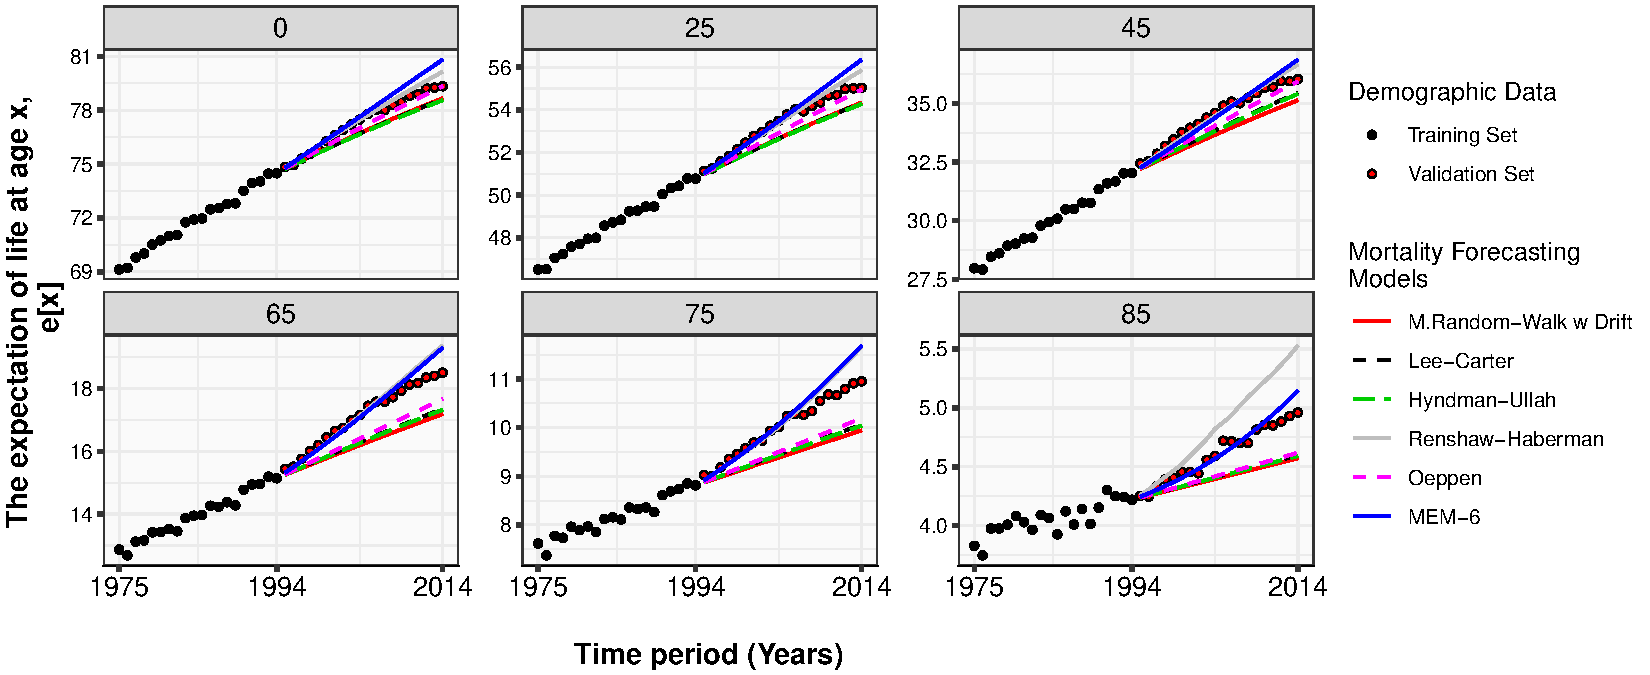
\includegraphics[width=1\linewidth]{figure/Figure_AUS_ex}
  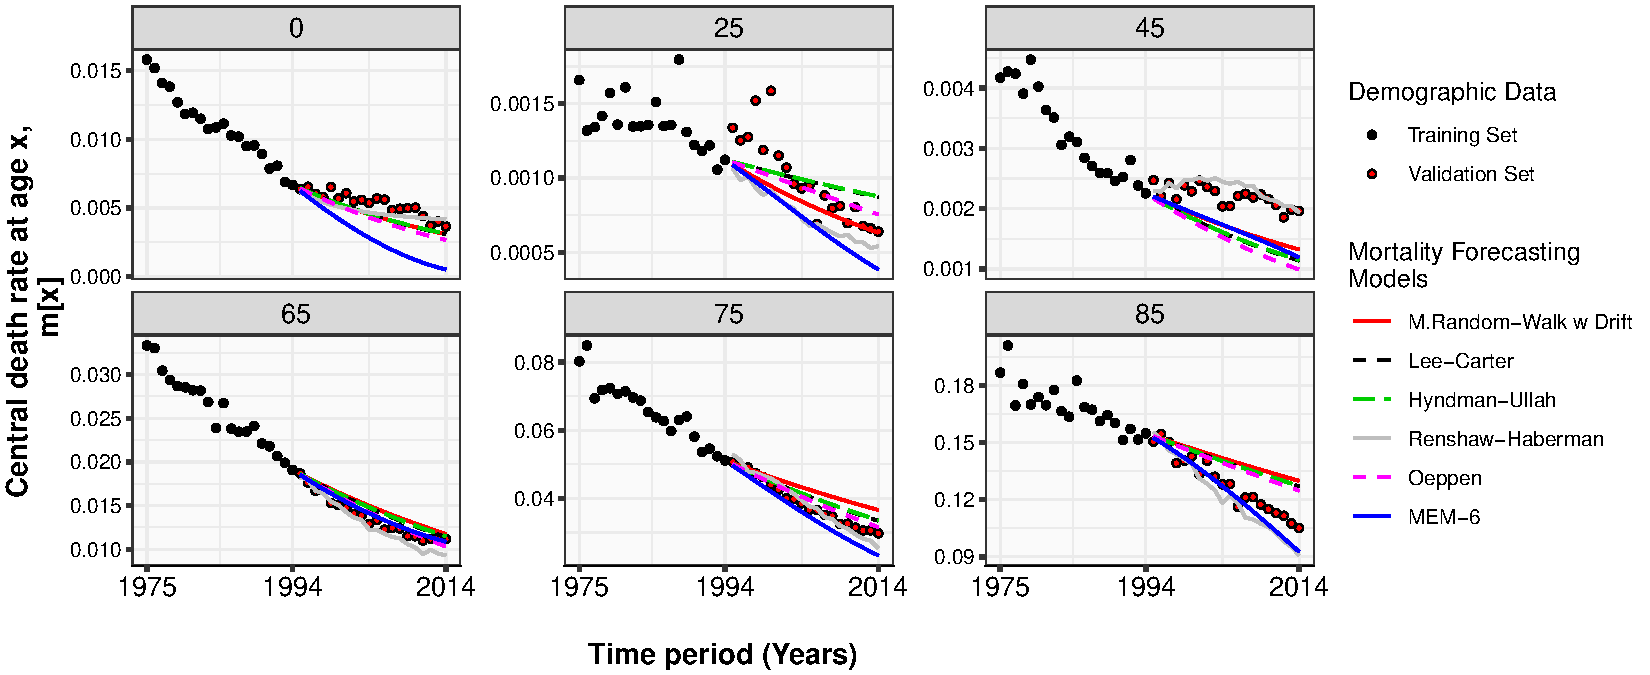
\includegraphics[width=1\linewidth]{figure/Figure_AUS_mx}
  \caption{Out-of-sample forecast of the remaining life expectancy and central death rates at various ages using the five mortality models (Australia, Male population, Scenario 16: 1975--1994--2014)}
\end{figure}

\newpage % ---------------------------
\subsection{Out-of-sample forecasts: Canada, Male population, 1960--2011}
\begin{table}[!ht]
\centering
\caption{Forecast accuracy measures aggregated over 13 scenarios in the 1960--2011 period} 
\label{tbl:res_CAN}
\scalebox{0.9}{
\begin{tabular}{lccccccc}
  \toprule
Model & ME & MAE & MAPE & sMAPE & sMRAE & MASE & GC \\ 
  \midrule
M.Random-Walk w Drift &  0.56 (5) & 0.57 (5) & 2.07 (4) & 2.10 (5) & 100.00 (5) & 3.58 (5) & (5) \\ 
  Lee-Carter &  0.60 (6) & 0.62 (6) & 2.25 (6) & 2.29 (6) & 104.39 (6) & 3.88 (6) & (6) \\ 
  Hyndman-Ullah &  0.44 (3) & 0.50 (3) & 1.98 (3) & 2.01 (3) &  92.82 (3) & 3.27 (3) & (3) \\ 
  Renshaw-Haberman &  0.12 (1) & 0.35 (2) & 1.55 (2) & 1.54 (2) &  83.31 (2) & 2.51 (2) & (2) \\ 
  Oeppen &  0.53 (4) & 0.55 (4) & 2.07 (5) & 2.10 (4) &  99.10 (4) & 3.52 (4) & (4) \\ 
  MEM-6 &  0.17 (2) & 0.26 (1) & 1.11 (1) & 1.12 (1) &  71.32 (1) & 1.81 (1) & (1) \\ 
   \bottomrule
\end{tabular}
}
\end{table}

\begin{figure}[!hb]
  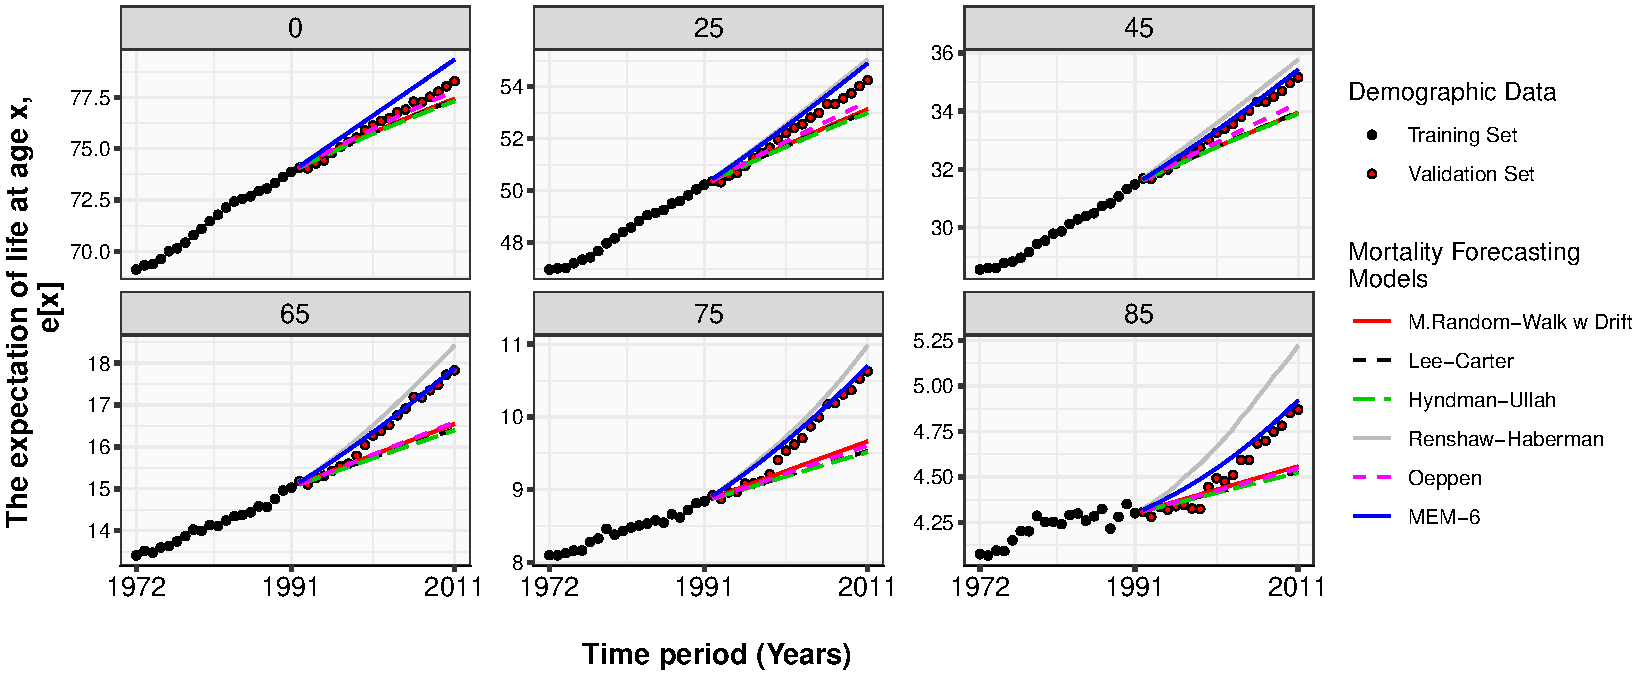
\includegraphics[width=1\linewidth]{figure/Figure_CAN_ex}
  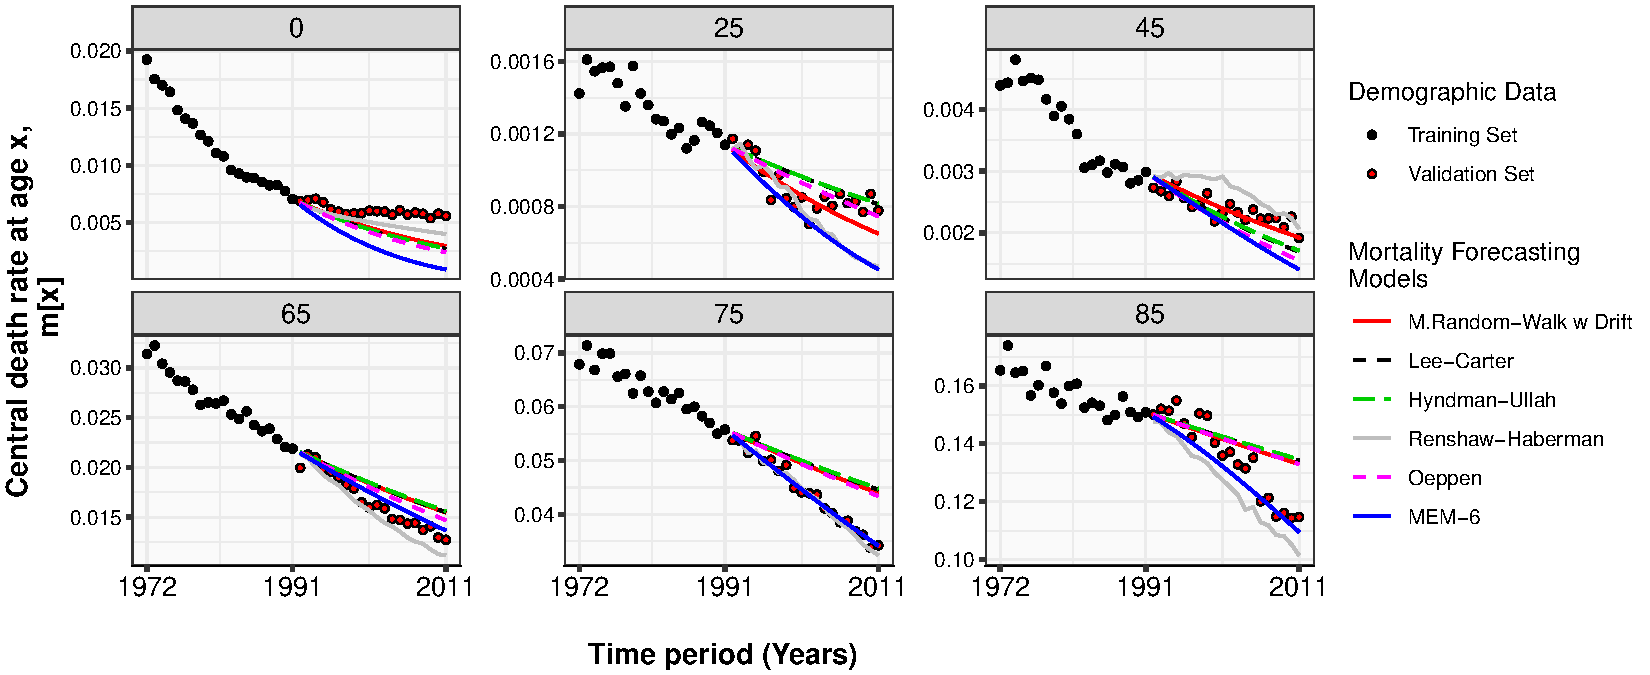
\includegraphics[width=1\linewidth]{figure/Figure_CAN_mx}
  \caption{Out-of-sample forecast of the remaining life expectancy and central death rates at various ages using the five mortality models (Canada, Male population, Scenario 13: 1972--1991--2011)}
\end{figure}

\newpage % ---------------------------
\subsection{Out-of-sample forecasts: France, Male population, 1960--2016}
\begin{table}[!ht]
\centering
\caption{Forecast accuracy measures aggregated over 18 scenarios in the 1960--2016 period} 
\label{tbl:res_FRATNP}
\scalebox{0.9}{
\begin{tabular}{lccccccc}
  \toprule
Model & ME & MAE & MAPE & sMAPE & sMRAE & MASE & GC \\ 
  \midrule
M.Random-Walk w Drift &  0.51 (6) & 0.53 (5) & 2.10 (5) & 2.14 (5) & 100.00 (5) & 3.47 (5) & (5) \\ 
  Lee-Carter &  0.49 (5) & 0.52 (4) & 1.90 (4) & 1.93 (3) &  96.00 (4) & 3.23 (4) & (3) \\ 
  Hyndman-Ullah &  0.47 (4) & 0.51 (3) & 1.90 (3) & 1.93 (4) &  93.75 (3) & 3.21 (3) & (3) \\ 
  Renshaw-Haberman &  0.44 (3) & 0.53 (6) & 2.37 (6) & 2.36 (6) & 101.03 (6) & 3.88 (6) & (6) \\ 
  Oeppen &  0.27 (1) & 0.38 (2) & 1.56 (1) & 1.58 (1) &  84.97 (1) & 2.51 (1) & (2) \\ 
  MEM-6 &  0.27 (2) & 0.38 (1) & 1.68 (2) & 1.69 (2) &  86.80 (2) & 2.61 (2) & (1) \\ 
   \bottomrule
\end{tabular}
}
\end{table}

\begin{figure}[!hb]
  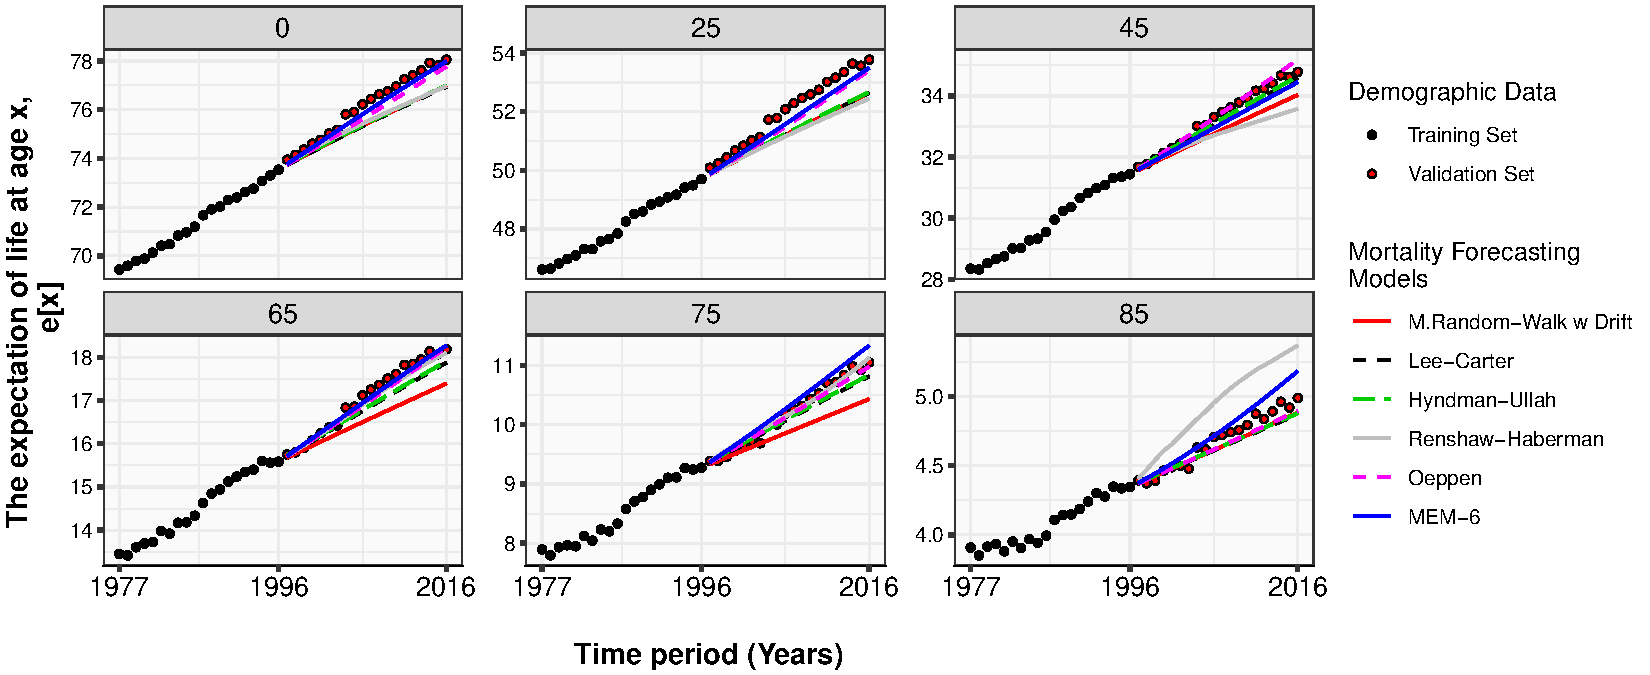
\includegraphics[width=1\linewidth]{figure/Figure_FRATNP_ex}
  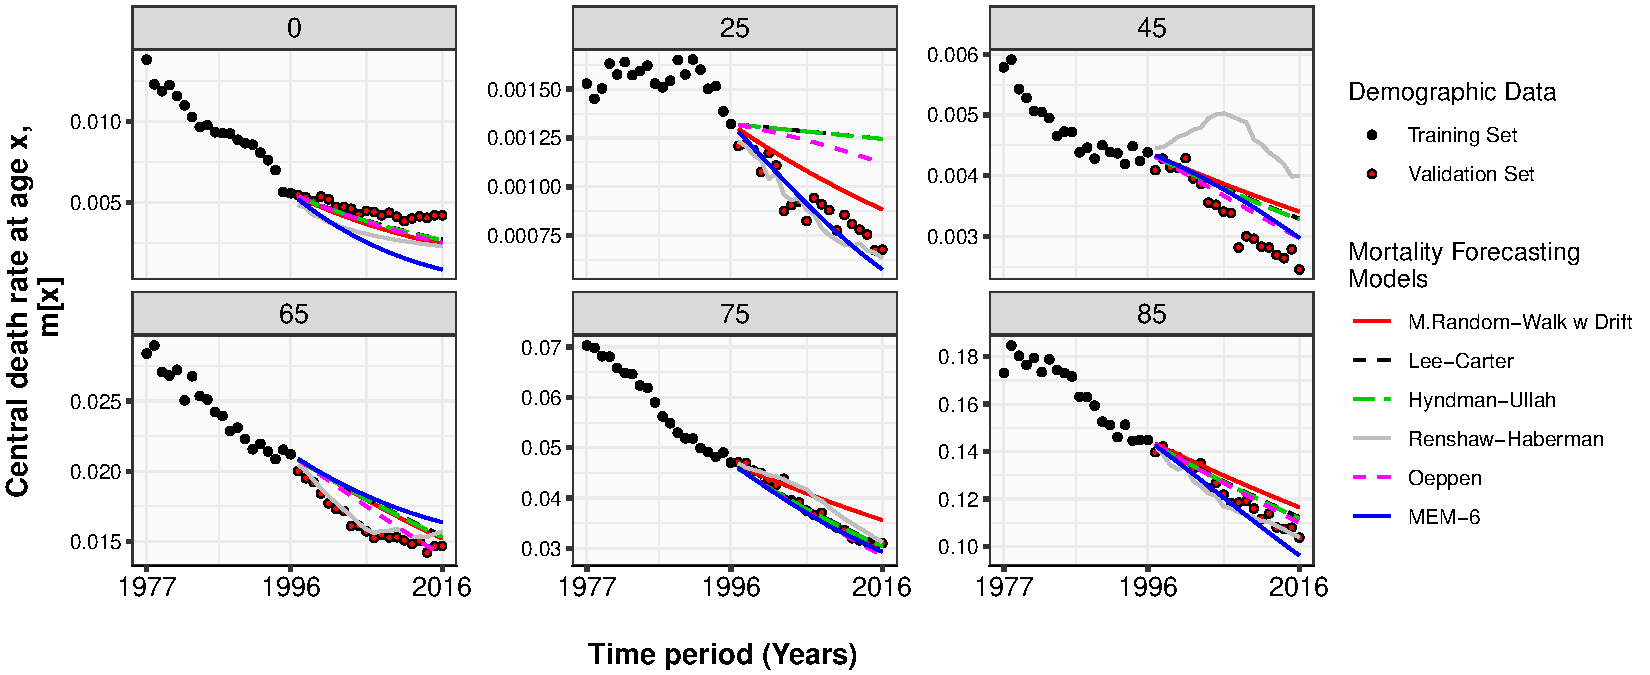
\includegraphics[width=1\linewidth]{figure/Figure_FRATNP_mx}
  \caption{Out-of-sample forecast of the remaining life expectancy and central death rates at various ages using the five mortality models (France, Male population, Scenario 18: 1977--1996--2016)}
\end{figure}

\newpage % ---------------------------
\subsection{Out-of-sample forecasts: Italy, Male population, 1960--2014}
\begin{table}[!ht]
\centering
\caption{Forecast accuracy measures aggregated over 16 scenarios in the 1960--2014 period} 
\label{tbl:res_ITA}
\scalebox{0.9}{
\begin{tabular}{lccccccc}
  \toprule
Model & ME & MAE & MAPE & sMAPE & sMRAE & MASE & GC \\ 
  \midrule
M.Random-Walk w Drift &  0.82 (4) & 0.83 (4) & 3.21 (4) & 3.30 (4) & 100.00 (4) & 4.64 (4) & (4) \\ 
  Lee-Carter &  0.92 (5) & 0.92 (5) & 3.40 (5) & 3.50 (5) & 103.97 (6) & 5.01 (5) & (5) \\ 
  Hyndman-Ullah &  0.92 (6) & 0.93 (6) & 3.41 (6) & 3.51 (6) & 103.79 (5) & 5.03 (6) & (6) \\ 
  Renshaw-Haberman &  0.54 (2) & 0.58 (2) & 2.53 (2) & 2.57 (2) &  85.64 (2) & 3.55 (2) & (2) \\ 
  Oeppen &  0.80 (3) & 0.80 (3) & 3.02 (3) & 3.10 (3) &  95.54 (3) & 4.40 (3) & (3) \\ 
  MEM-5 &  0.37 (1) & 0.41 (1) & 2.01 (1) & 2.06 (1) &  71.72 (1) & 2.58 (1) & (1) \\ 
   \bottomrule
\end{tabular}
}
\end{table}

\begin{figure}[!hb]
  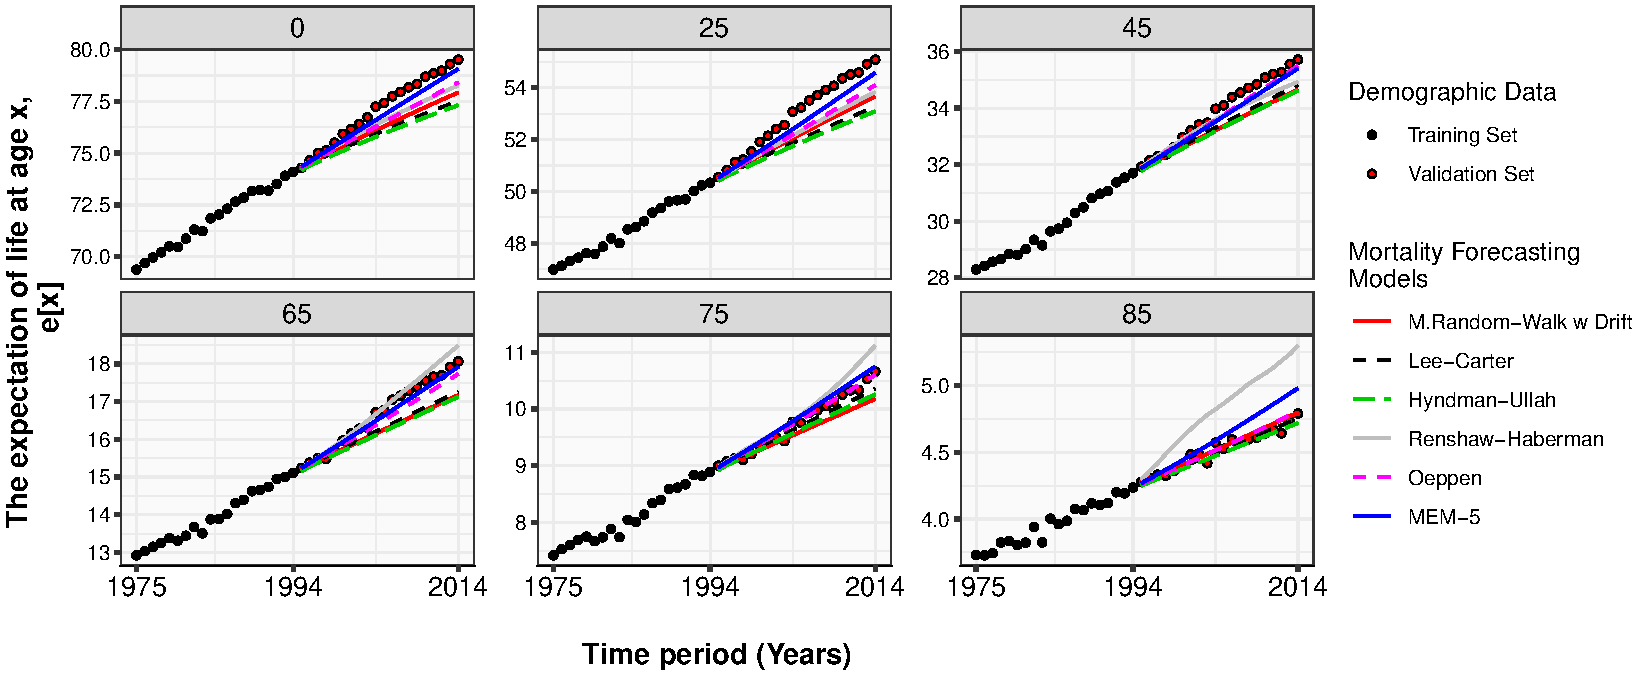
\includegraphics[width=1\linewidth]{figure/Figure_ITA_ex}
  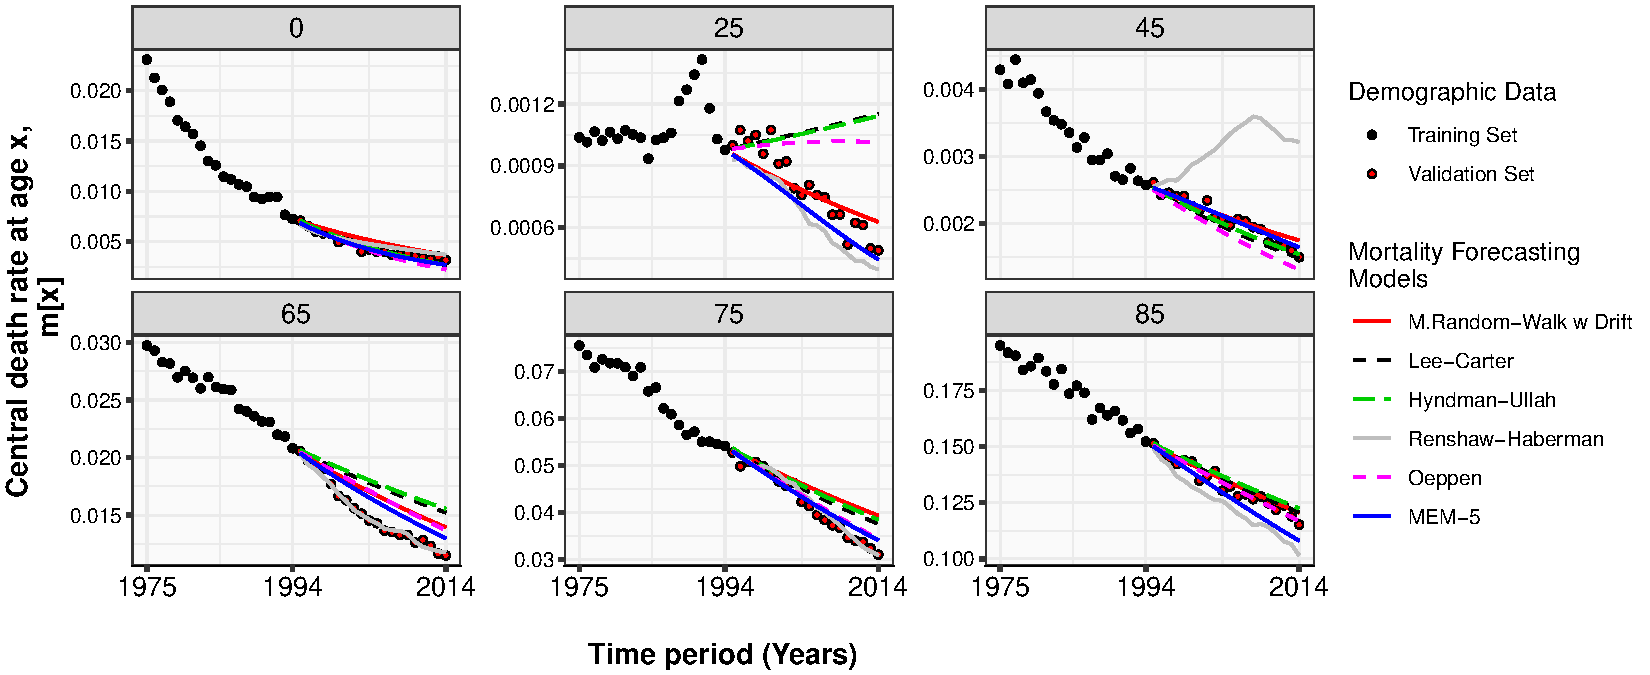
\includegraphics[width=1\linewidth]{figure/Figure_ITA_mx}
  \caption{Out-of-sample forecast of the remaining life expectancy and central death rates at various ages using the five mortality models (Italy, Male population, Scenario 16: 1975--1994--2014)}
\end{figure}

\newpage % ---------------------------
\subsection{Out-of-sample forecasts: The Netherlands, Male population, 1960--2016}
\begin{table}[!ht]
\centering
\caption{Forecast accuracy measures aggregated over 18 scenarios in the 1960--2016 period} 
\label{tbl:res_NLD}
\scalebox{0.9}{
\begin{tabular}{lccccccc}
  \toprule
Model & ME & MAE & MAPE & sMAPE & sMRAE & MASE & GC \\ 
  \midrule
M.Random-Walk w Drift & 0.75 (3) & 0.77 (3) & 2.99 (3) & 3.07 (3) & 100.00 (3) & 4.55 (3) & (3) \\ 
  Lee-Carter & 0.79 (6) & 0.81 (6) & 3.23 (5) & 3.33 (5) & 104.27 (5) & 4.88 (6) & (6) \\ 
  Hyndman-Ullah & 0.79 (5) & 0.81 (5) & 3.24 (6) & 3.33 (6) & 104.37 (6) & 4.88 (5) & (5) \\ 
  Renshaw-Haberman & 0.30 (1) & 0.36 (1) & 1.48 (1) & 1.49 (1) &  70.61 (1) & 2.22 (1) & (1) \\ 
  Oeppen & 0.77 (4) & 0.80 (4) & 3.19 (4) & 3.29 (4) & 103.62 (4) & 4.80 (4) & (4) \\ 
  MEM-5 & 0.59 (2) & 0.62 (2) & 2.53 (2) & 2.59 (2) &  90.04 (2) & 3.81 (2) & (2) \\ 
   \bottomrule
\end{tabular}
}
\end{table}

\begin{figure}[!hb]
  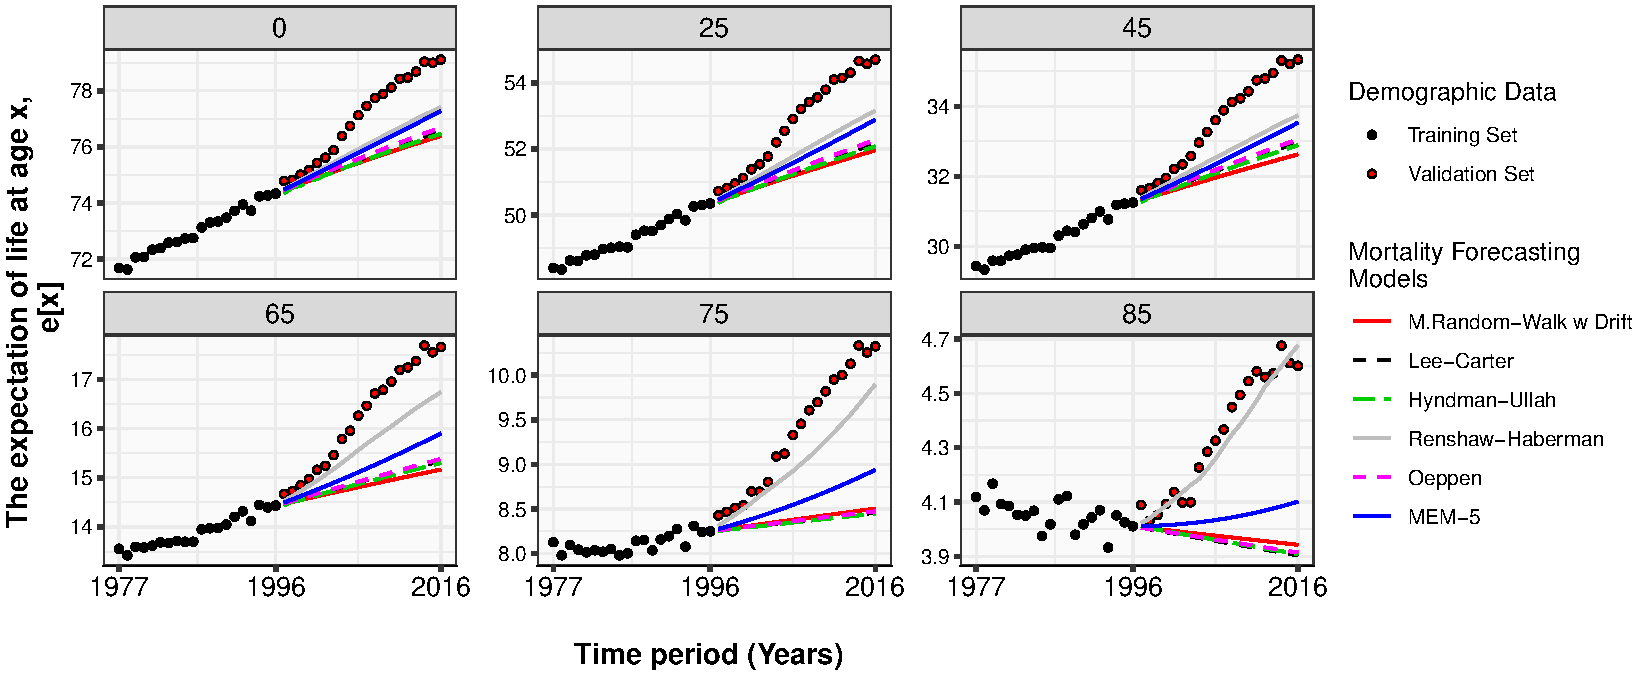
\includegraphics[width=1\linewidth]{figure/Figure_NLD_ex}
  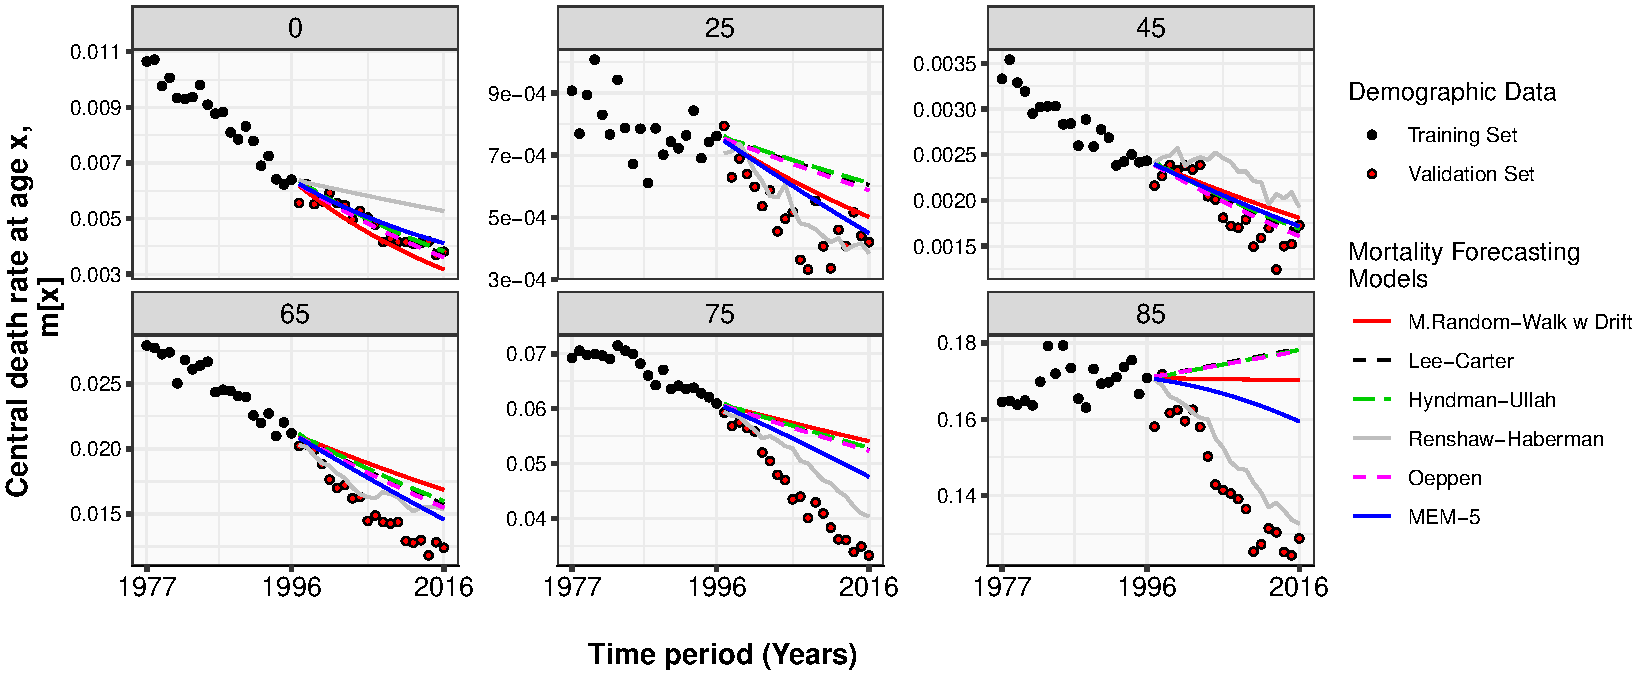
\includegraphics[width=1\linewidth]{figure/Figure_NLD_mx}
  \caption{Out-of-sample forecast of the remaining life expectancy and central death rates at various ages using the five mortality models (The Netherlands, Male population, Scenario 18: 1977--1996--2016)}
\end{figure}

\newpage % ---------------------------
\subsection{Out-of-sample forecasts: Spain, Male population, 1960--2014}
\begin{table}[!ht]
\centering
\caption{Forecast accuracy measures aggregated over 16 scenarios in the 1960--2014 period} 
\label{tbl:res_ESP}
\scalebox{0.9}{
\begin{tabular}{lccccccc}
  \toprule
Model & ME & MAE & MAPE & sMAPE & sMRAE & MASE & GC \\ 
  \midrule
M.Random-Walk w Drift &  0.12 (2) & 0.31 (1) &  1.35 (3) &  1.34 (3) & 100.00 (3) &  2.28 (3) & (3) \\ 
  Lee-Carter &  0.09 (1) & 0.34 (2) &  1.17 (1) &  1.17 (1) &  97.62 (1) &  2.19 (1) & (1) \\ 
  Hyndman-Ullah &  0.13 (3) & 0.34 (3) &  1.18 (2) &  1.18 (2) &  97.72 (2) &  2.21 (2) & (2) \\ 
  Renshaw-Haberman &  0.45 (6) & 0.84 (6) &  3.44 (6) &  4.65 (6) & 114.59 (6) &  6.14 (6) & (6) \\ 
  Oeppen & -0.14 (4) & 0.37 (4) &  1.38 (4) &  1.37 (4) & 105.86 (4) &  2.54 (4) & (4) \\ 
  MEM-5 & -0.30 (5) & 0.50 (5) &  1.65 (5) &  1.63 (5) & 111.11 (5) &  3.42 (5) & (5) \\ 
   \bottomrule
\end{tabular}
}
\end{table}

\begin{figure}[!hb]
  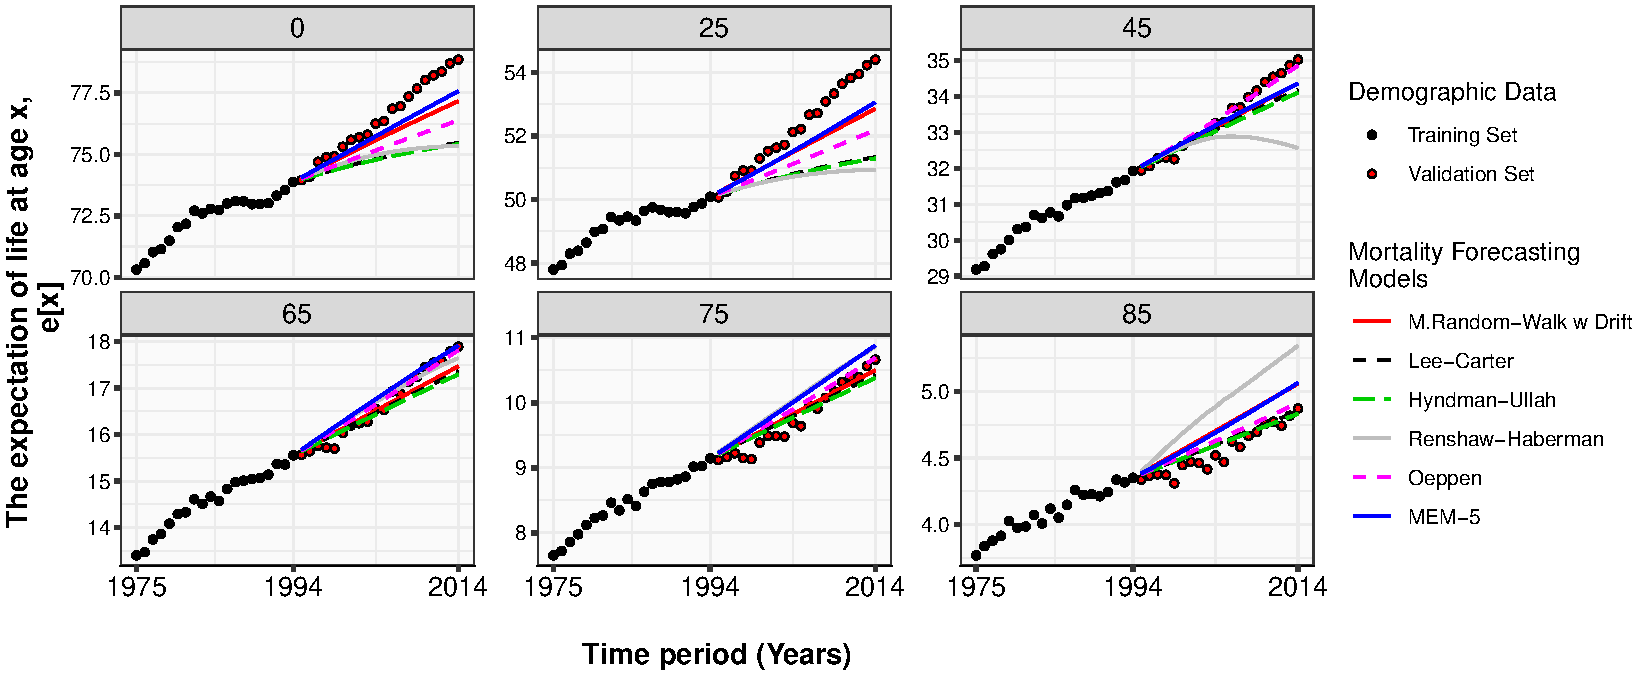
\includegraphics[width=1\linewidth]{figure/Figure_ESP_ex}
  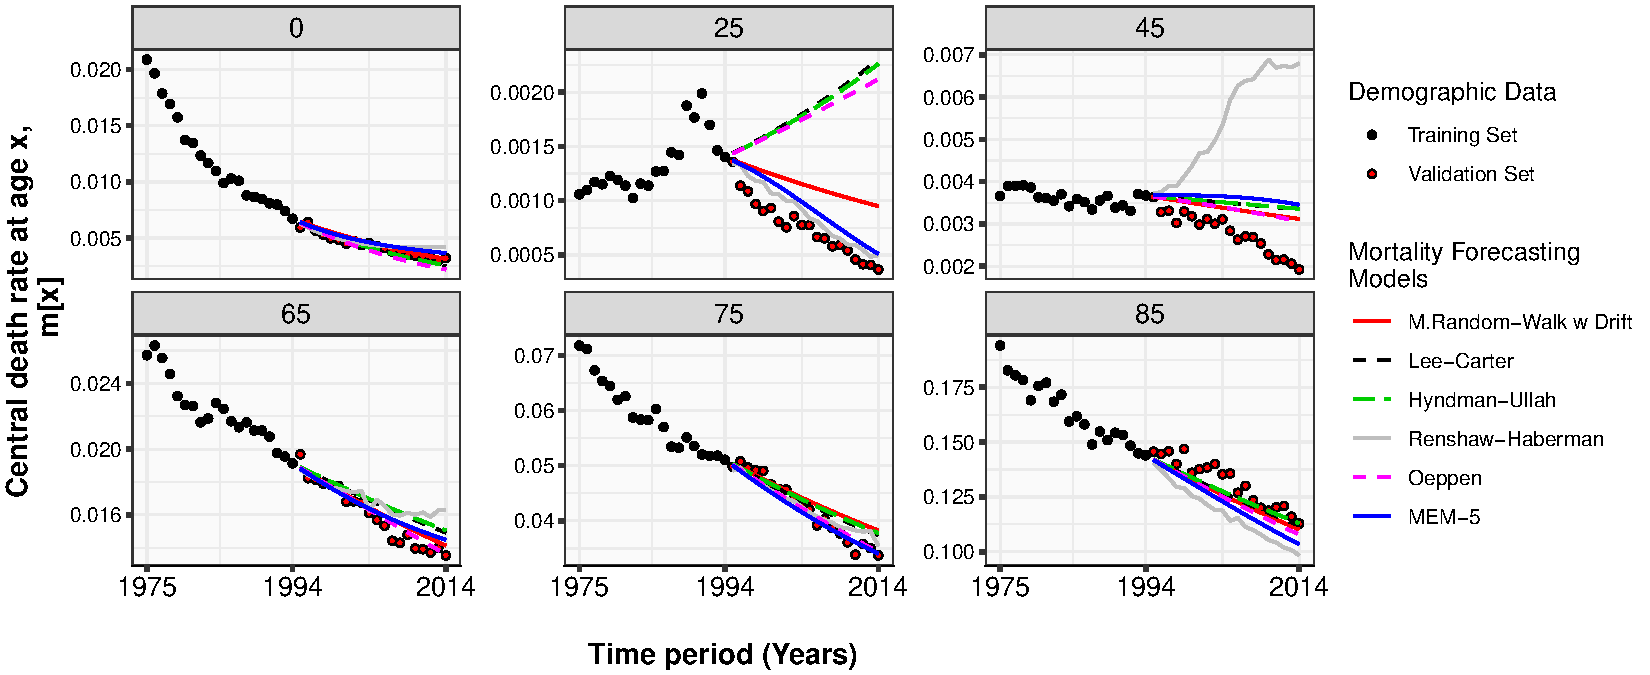
\includegraphics[width=1\linewidth]{figure/Figure_ESP_mx}
  \caption{Out-of-sample forecast of the remaining life expectancy and central death rates at various ages using the five mortality models (Spain, Male population, Scenario 16: 1975--1994--2014)}
\end{figure}

\newpage % ---------------------------
\subsection{Out-of-sample forecasts: Switzerland, Male population, 1960--2016}
\begin{table}[!ht]
\centering
\caption{Forecast accuracy measures aggregated over 18 scenarios in the 1960--2016 period} 
\label{tbl:res_CHE}
\scalebox{0.9}{
\begin{tabular}{lccccccc}
  \toprule
Model & ME & MAE & MAPE & sMAPE & sMRAE & MASE & GC \\ 
  \midrule
M.Random-Walk w Drift &  0.58 (3) &  0.61 (3) &  2.19 (4) &  2.22 (4) & 100.00 (4) &  3.34 (3) & (3) \\ 
  Lee-Carter &  0.62 (4) &  0.64 (4) &  2.17 (3) &  2.20 (3) & 100.91 (5) &  3.43 (4) & (3) \\ 
  Hyndman-Ullah &  0.66 (5) &  0.68 (5) &  2.30 (5) &  2.34 (5) & 106.15 (6) &  3.65 (5) & (6) \\ 
  Renshaw-Haberman &  1.13 (6) &  1.23 (6) &  4.24 (6) &  6.45 (6) &  93.44 (3) &  6.69 (6) & (5) \\ 
  Oeppen &  0.45 (2) &  0.50 (2) &  1.74 (2) &  1.76 (2) &  89.54 (2) &  2.69 (2) & (2) \\ 
  MEM-5 &  0.35 (1) &  0.40 (1) &  1.41 (1) &  1.42 (1) &  81.59 (1) &  2.17 (1) & (1) \\ 
   \bottomrule
\end{tabular}
}
\end{table}

\begin{figure}[!hb]
  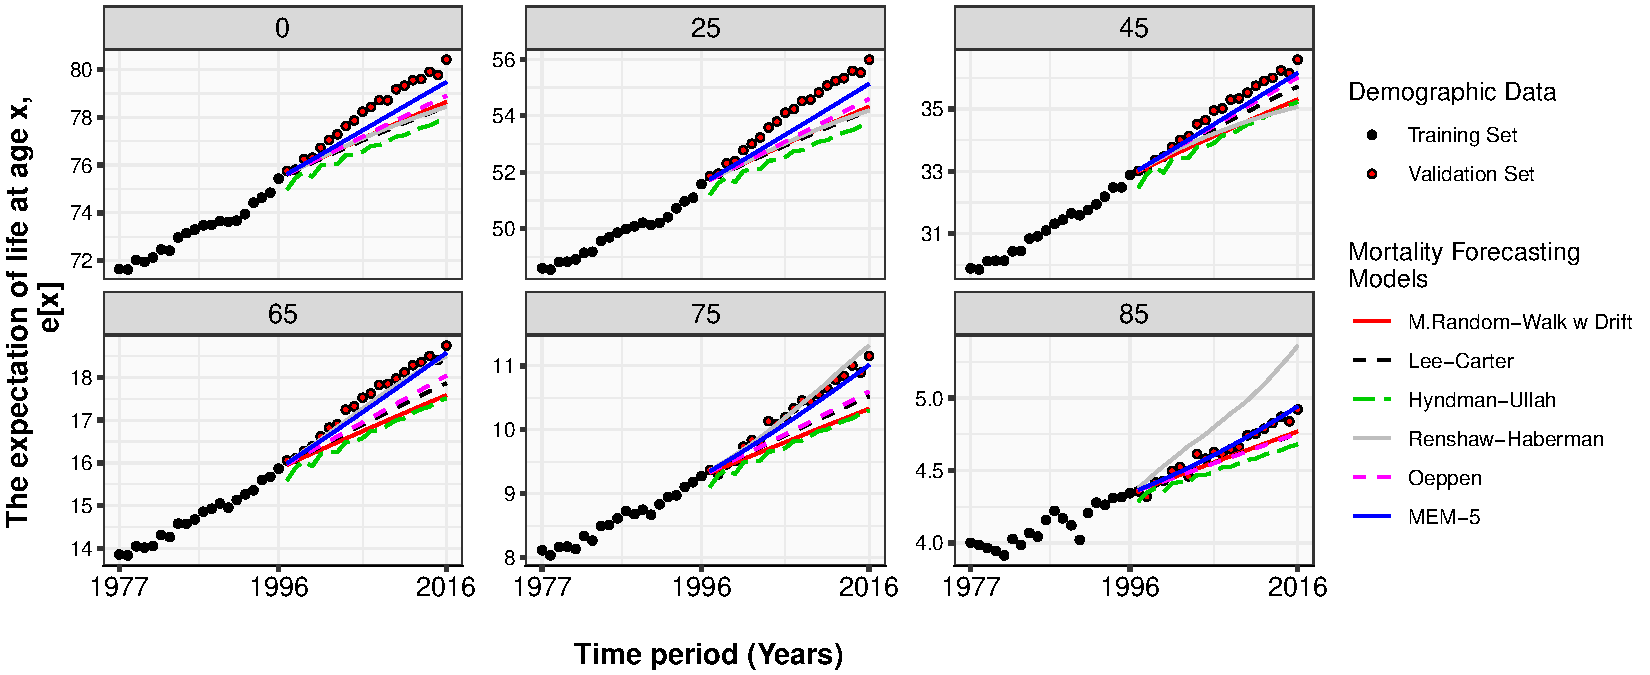
\includegraphics[width=1\linewidth]{figure/Figure_CHE_ex}
  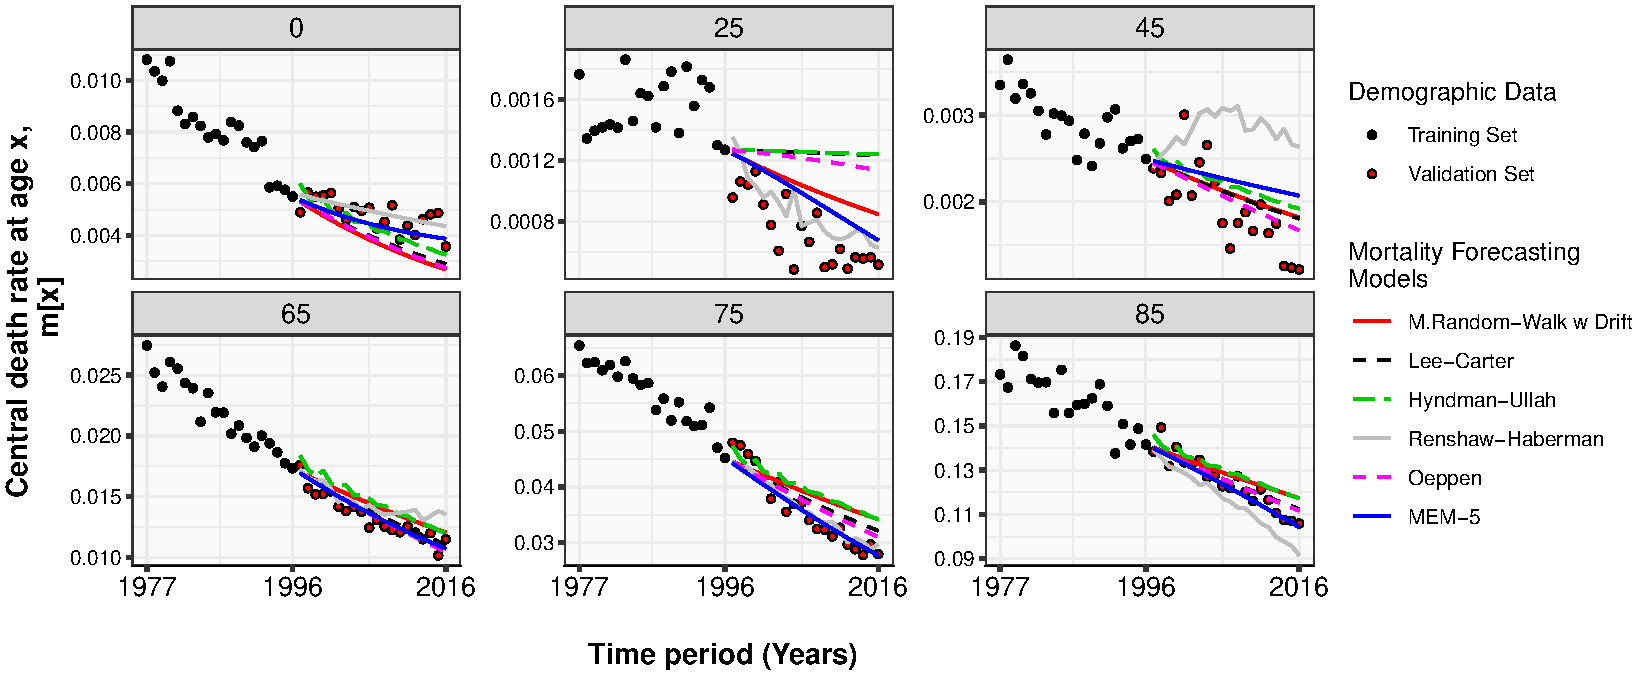
\includegraphics[width=1\linewidth]{figure/Figure_CHE_mx}
  \caption{Out-of-sample forecast of the remaining life expectancy and central death rates at various ages using the five mortality models (Switzerland, Male population, Scenario 18: 1977--1996--2016)}
\end{figure}

\newpage % ---------------------------
\subsection{Out-of-sample forecasts: Sweden, Male population, 1960--2016}
\begin{table}[!ht]
\centering
\caption{Forecast accuracy measures aggregated over 18 scenarios in the 1960--2016 period} 
\label{tbl:res_SWE}
\scalebox{0.9}{
\begin{tabular}{lccccccc}
  \toprule
Model & ME & MAE & MAPE & sMAPE & sMRAE & MASE & GC \\ 
  \midrule
M.Random-Walk w Drift &  0.85 (4) & 0.86 (4) & 3.02 (4) & 3.09 (4) & 100.00 (5) & 5.24 (4) & (4) \\ 
  Lee-Carter &  0.87 (5) & 0.88 (5) & 3.06 (5) & 3.13 (5) &  98.85 (4) & 5.33 (5) & (5) \\ 
  Hyndman-Ullah &  0.92 (6) & 0.92 (6) & 3.19 (6) & 3.28 (6) & 104.01 (6) & 5.60 (6) & (6) \\ 
  Renshaw-Haberman &  0.68 (1) & 0.72 (2) & 2.70 (2) & 2.75 (2) &  86.45 (1) & 4.49 (2) & (1) \\ 
  Oeppen &  0.81 (3) & 0.82 (3) & 2.87 (3) & 2.94 (3) &  93.12 (3) & 4.98 (3) & (3) \\ 
  MEM-5 &  0.68 (2) & 0.70 (1) & 2.54 (1) & 2.60 (1) &  86.90 (2) & 4.26 (1) & (1) \\ 
   \bottomrule
\end{tabular}
}
\end{table}

\begin{figure}[!hb]
  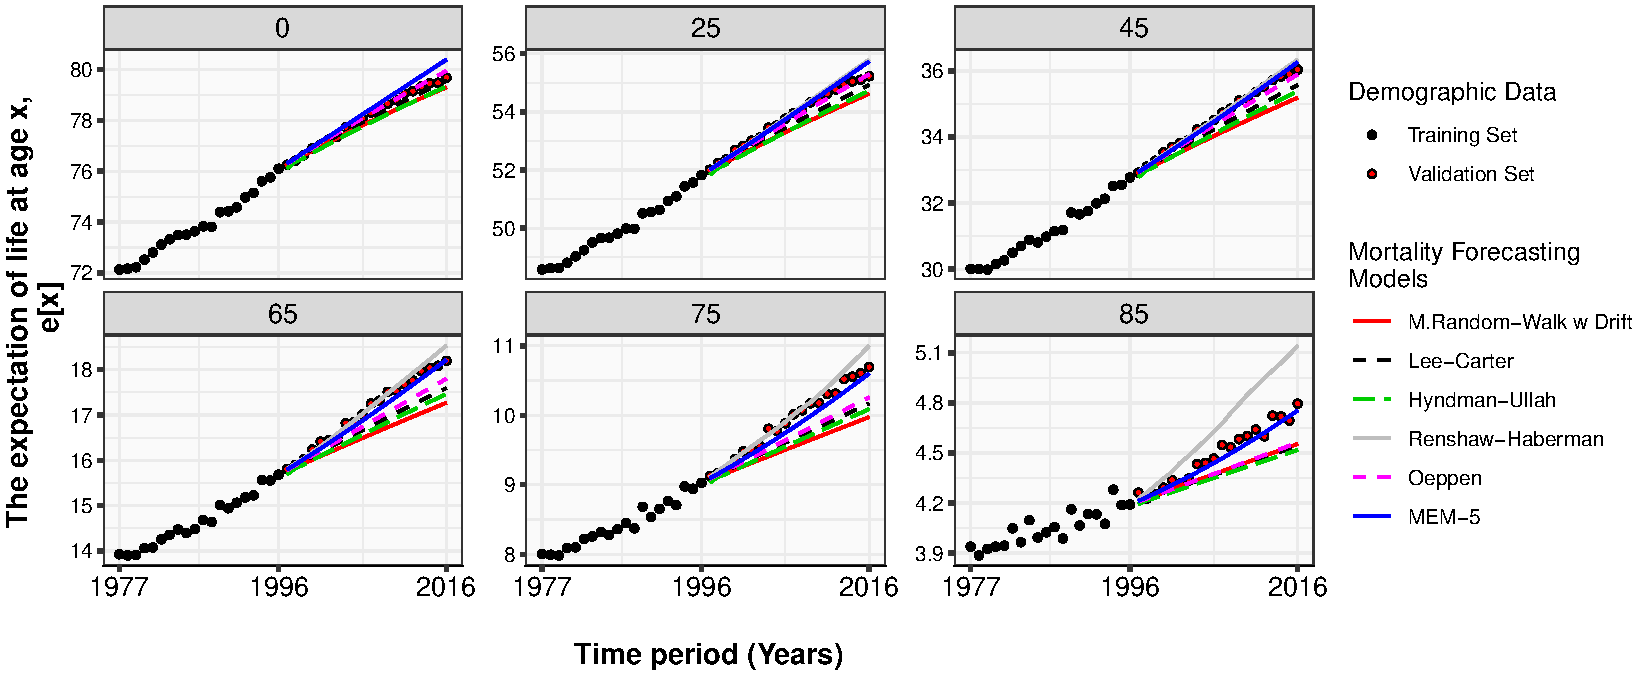
\includegraphics[width=1\linewidth]{figure/Figure_SWE_ex}
  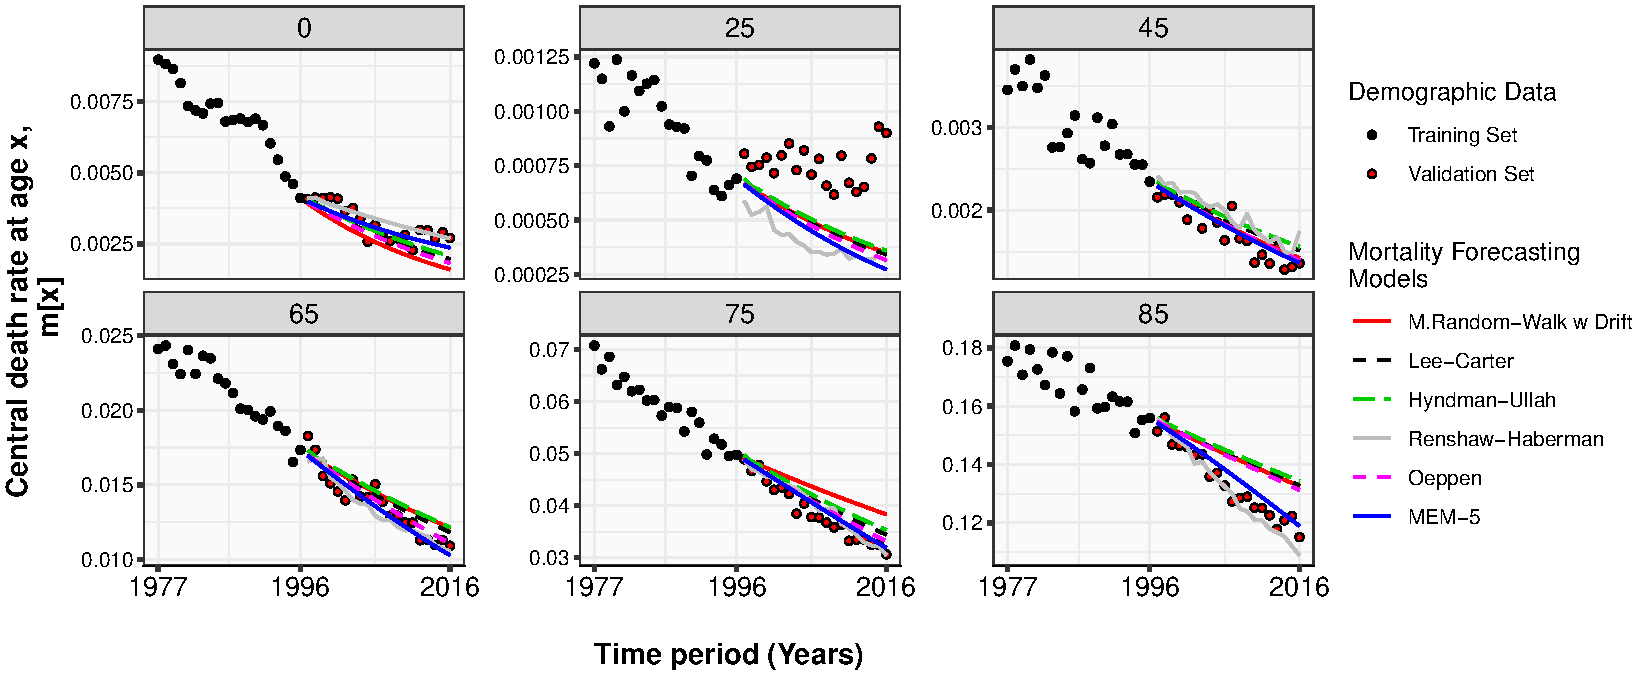
\includegraphics[width=1\linewidth]{figure/Figure_SWE_mx}
  \caption{Out-of-sample forecast of the remaining life expectancy and central death rates at various ages using the five mortality models (Sweden, Male population, Scenario 18: 1977--1996--2016)}
\end{figure}

\newpage % ---------------------------
\subsection{Out-of-sample forecasts: USA, Male population, 1960--2016}
\begin{table}[!ht]
\centering
\caption{Forecast accuracy measures aggregated over 18 scenarios in the 1960--2016 period} 
\label{tbl:res_USA}
\scalebox{0.9}{
\begin{tabular}{lccccccc}
  \toprule
Model & ME & MAE & MAPE & sMAPE & sMRAE & MASE & GC \\ 
  \midrule
M.Random-Walk w Drift &  0.24 (5) &  0.30 (4) &  1.32 (4) &   1.33 (4) & 100.00 (4) &   2.57 (4) & (4) \\ 
  Lee-Carter &  0.23 (4) &  0.30 (3) &  1.29 (3) &   1.31 (3) &  98.69 (3) &   2.51 (3) & (3) \\ 
  Hyndman-Ullah &  0.15 (3) &  0.42 (5) &  1.76 (5) &   1.78 (5) & 111.15 (5) &   3.49 (5) & (5) \\ 
  Renshaw-Haberman &  2.84 (6) &  3.35 (6) & 12.37 (6) &  21.27 (6) & 126.88 (6) &  27.97 (6) & (6) \\ 
  Oeppen &  0.09 (1) &  0.22 (1) &  1.07 (2) &   1.08 (2) &  87.29 (1) &   2.04 (2) & (1) \\ 
  MEM-6 & -0.10 (2) &  0.24 (2) &  1.03 (1) &   1.02 (1) &  92.31 (2) &   2.03 (1) & (2) \\ 
   \bottomrule
\end{tabular}
}
\end{table}

\begin{figure}[!hb]
  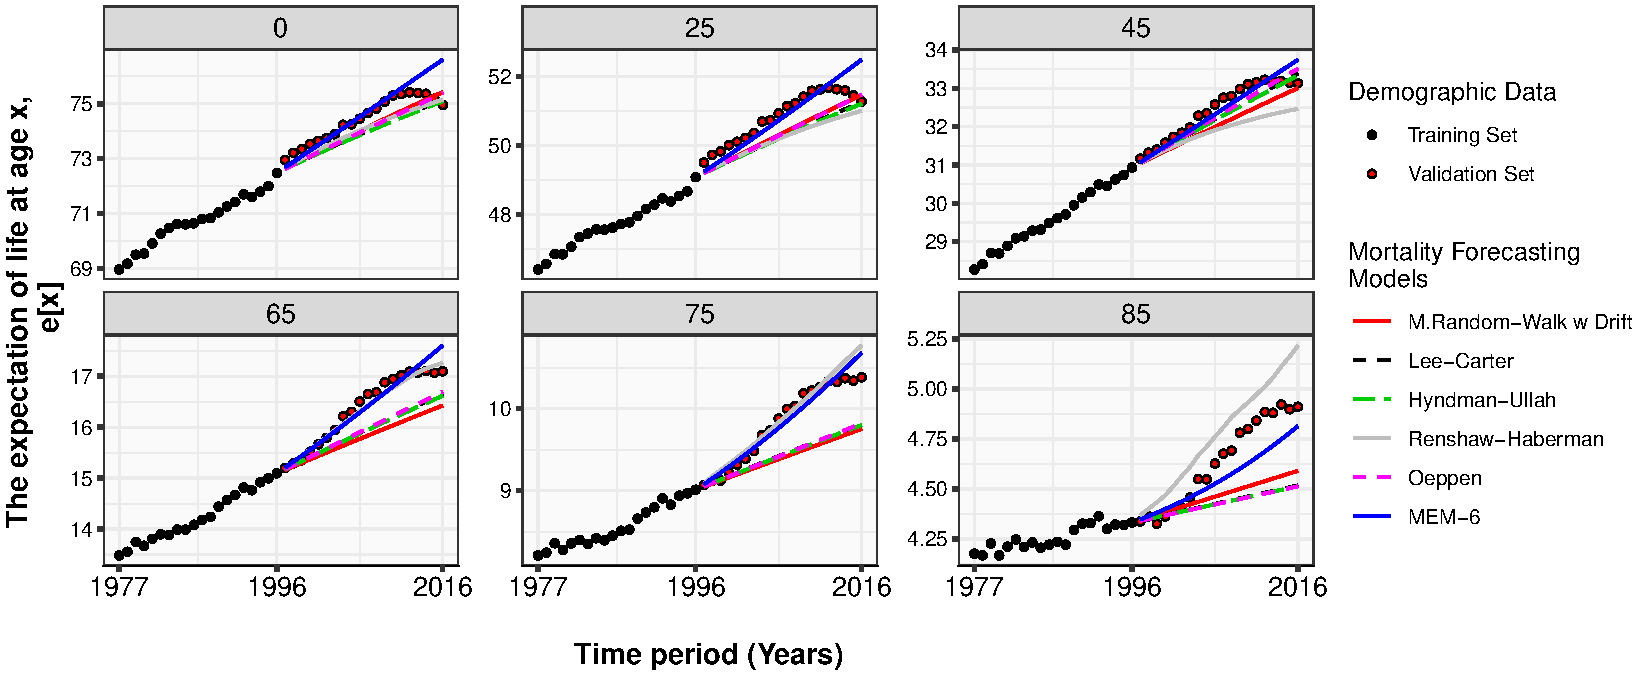
\includegraphics[width=1\linewidth]{figure/Figure_USA_ex}
  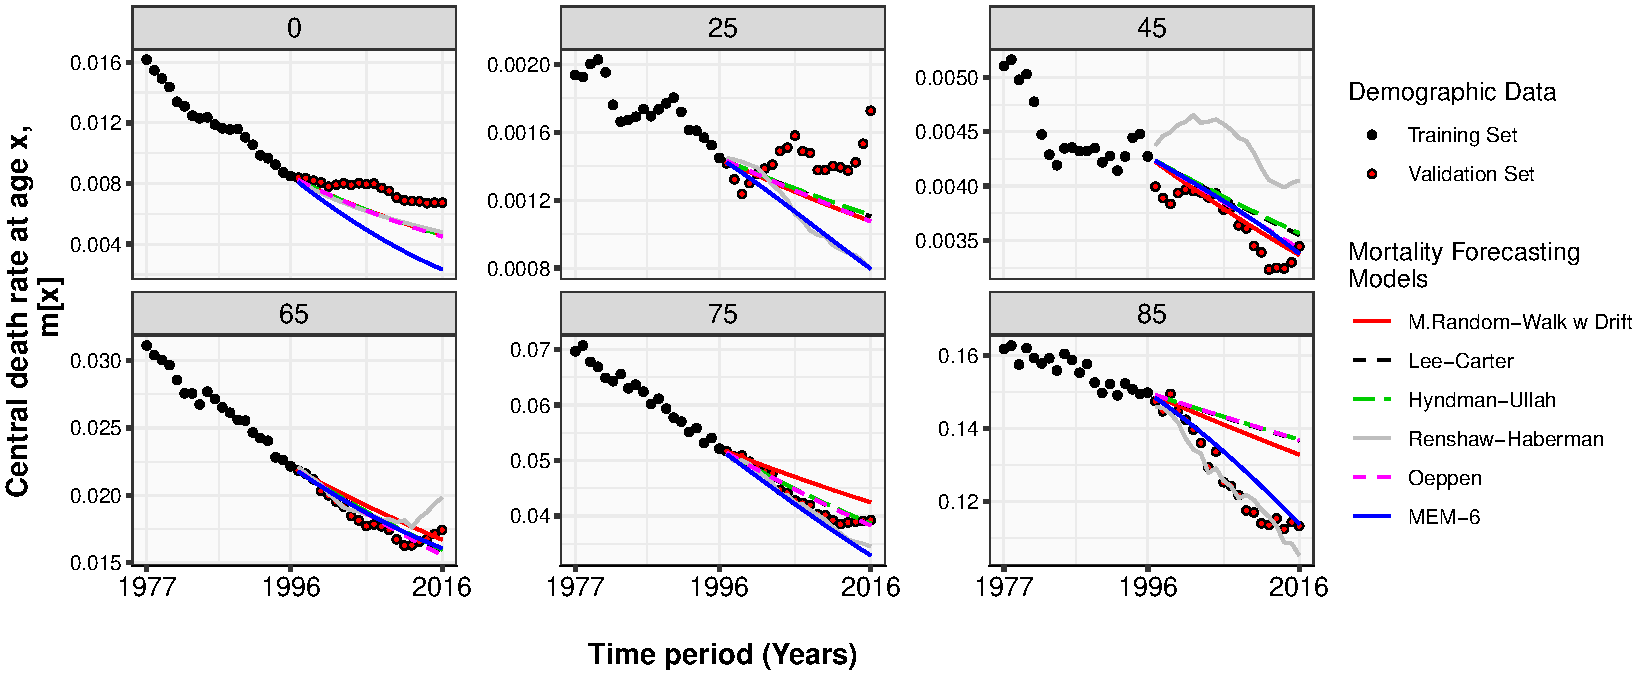
\includegraphics[width=1\linewidth]{figure/Figure_USA_mx}
  \caption{Out-of-sample forecast of the remaining life expectancy and central death rates at various ages using the five mortality models (USA, Male population, Scenario 18: 1977--1996--2016)}
\end{figure}

\newpage
\end{document}